\documentclass[]{article}

\usepackage[colorlinks=true]{hyperref}
\usepackage{amssymb}
\usepackage{graphicx}
\usepackage{subcaption}

\author{Robin Deits}
\date{\today}
\title{Internet of Toys: Julia and Lego Mindstorms}

\newcommand{\ev}{\textsc{ev3}}

\begin{document}
\maketitle

\abstract{%
The latest version of the Lego Mindstorms robotics system is an excellent candidate for the exploration of distributed robotics. I implemented bindings to the \texttt{ev3dev} operating system, which runs on the Mindstorms \textsc{ev3} brick, in Julia. Using those bindings, I constructed a library to perform a simple cooperative mapping task on a pair of mobile robots. Due to the hardware limitations of the \textsc{ev3} processor, I was not yet able to run Julia onboard. Instead, I developed a simple server-client architecture using ZeroMQ \cite{hintjens_zeromq:_2015} to allow Julia code to run off-board and control the Mindstorms robot over WiFi. With this system, I was able to map simple environments both in serial (with one robot) and in parallel (with a team of two robots).%
}

\tableofcontents

\section{Background}
The Lego Mindstorms system was first released in 1998, with the Mindstorms Robotics Invention System \cite{the_lego_group_history_2015}. The Mindstorms system consists of a central computer with input and output ports, and a set of lego-compatible motors and sensors, as seen in Fig. \ref{fig:mindstorms_bricks}. Lego provides a development environment for the Mindstorms computer, in which users can create programs using a visual block language. There have been a variety of attempts to introduce more traditional programming languages to the Mindstorms environment, including Not Quite C \cite{_not_2007} and Next Byte Codes \cite{_next_2011}. These efforts have focused on writing and compiling code on a user's PC, and then deploying that code to the Mindstorms computer for execution, since the software on the Mindstorms brick was proprietary and closed. 

\begin{figure}[hb!]
    \centering
    \begin{subfigure}[htbp]{0.4\textwidth}
        \includegraphics[width=\textwidth]{fig/RCX-connections.png}
        \caption{The original 1998 Mindstorms \textsc{rcx}, with sensors and motors attached.}
        \label{fig:rcx}
    \end{subfigure}
    \qquad
    \begin{subfigure}[htbp]{0.4\textwidth}
        \includegraphics[width=\textwidth]{fig/ev3_connections.jpg}
        \caption{The 2013 Mindstorms \ev{}, with motors and sensors.}
        \label{fig:ev3}
    \end{subfigure}
    \caption{The Lego Mindstorms computer bricks, with attached peripherals. Figures reproduced from \cite{_legomindstormsrobots.com_2015}.}
    \label{fig:mindstorms_bricks}
\end{figure}


Fortunately, the situation has been radically improved with the newest Lego Mindstorms release, \ev{}. With \ev{}, the brick (the box which houses the battery, computer, screen, and interface ports) is now a small Linux computer complete with USB and MicroSD ports. This means that it is now possible to install and even develop software directly on the \ev{} using standard Linux tools. Even better, the \ev{} is capable of booting directly from the MicroSD port, which opens the door for custom operating systems. 

I have built my work on top of ev3dev, a custom Debian Linux distribution built specifically to run on the \ev{}. The ev3dev distro makes communicating with the basic \ev{} hardware particularly easy by mapping sensors and motors directly to nodes in the filesystem. For example, instructing a motor to run continuously is as simple as:
\begin{verbatim}
    echo run-forever > /sys/class/tacho-motor/motor2/command
\end{verbatim}
The developers of ev3dev also provide higher level bindings for C++, Python, Lua, and node.js. Rather than building Julia wrappers for any of these language bindings, I have written a new set of bindings directly on top of the filesystem interface provided by the ev3dev OS. 

\section{Hardware Interface}

\subsection{Running Julia on the EV3}

Creating a working build of Julia on the \ev{} proved to be much more difficult than anticipated, and I was not able to cross-compile a usable version. The \ev{} has an older ARM926EJ-S processor running the \texttt{ARMv5} instruction set. Although Julia has been successfully built on other ARM devices like the Raspberry Pi, the \ev{} is more limited in three ways:

\begin{enumerate}
\item Instruction set: The \ev{} uses the older ARMv5 instruction set. Julia has been built on systems using ARMv6 and ARMv7, but never yet on v5 \cite{_building_2015}.
\item Floating-point support: The \ev{} processor has no hardware floating-point support, and instead relies on the compiler to emulate floating-point operations in software. Julia does not have built-in support for so-called ``soft floating-point'' CPUs. 
\item Available RAM: The \ev{} has only 64\,MB of RAM, which may be enough to run Julia, but is not enough to compile its dependencies (particularly LLVM). 
\end{enumerate} 

Since the resources on the \ev{} were limited to a 300\,MHz processor and 64\,MB of RAM, I was forced to resort to cross-compilation to build Julia. Using the Brickstrap toolchain \cite{_brickstrap_2015}, I was able to build a complete image of the \texttt{ev3dev} operating system and compile Julia within Brickstrap but was never able to run the resulting Julia build without segmentation faults on startup. More discussion of the specific technical issues encountered can be seen in the discussion on the \texttt{julia-dev} mailing list in \cite{deits_building_2015}. 

Despite these setbacks, it is not yet clear that Julia cannot be built on the \ev{}. I plan to continue experimenting with Julia, specifically by attempting to identify and remove components of Julia which are failing on the \ev{}. 

\subsection{Running Julia Off-board}

\begin{figure}[thpb]
\centering
    \includegraphics[width=\textwidth, clip=true, trim=0 0 0 4.5in]{fig/offboard_arch.pdf}
    \caption{System architecture for controlling the Mindstorms \ev{} from a separate computer in Julia. ZeroMQ is used as a communication layer over WiFi to emulate the process of running Julia directly on the \ev{}}
    \label{fig:offboard}
\end{figure}

Without a working Julia build on the \ev{}, I decided to create a minimal system to allow Julia to run on an off-board PC while still communicating with the \ev{}'s sensors and motors. The easiest way to do this would be to mount the virtual file system provided by \texttt{ev3dev} on the user's PC, using a tool like AFS or SSHFS. I implemented the SSHFS mount, but experienced very poor reliability, with many commands being dropped or intermittently ignored. It appeared that the unreliable WiFi connection to the \ev{} made mounting a stable remote filesystem too difficult. 

Instead, I chose to use ZeroMQ \cite{hintjens_zeromq:_2015}, a robust, high-performance communication library to transmit messages between the \ev{} and the host PC. In all of my experiments, ZeroMQ was remarkably reliable, surviving network dropouts and various software crashes without issue. The structure of the system can be seen in Fig. \ref{fig:offboard}. On the \ev{}, a small Python program acts as a server using a ZeroMQ socket. The Python server listens for messages containing one of three commands: \texttt{r}, \texttt{w}, and \texttt{l} to read, write, or list, respectively, files on the device. Since all motors and sensors are mapped to files in \texttt{ev3dev}, those commands are all that are needed for full remote control of the \ev{}. The Python server also caches the handles to these virtual files in order to allow faster access to the hardware devices. 

In Julia, a few helper classes abstract away the ZeroMQ layer in order to make running off-board similar to running directly on the \ev{}. The \texttt{AbstractNode} type represents a file or directory on a local or remote filesystem. Its subtypes, \texttt{LocalNode} and \texttt{RemoteNode} contain the implementation details for a particular real file. In the case of a \texttt{LocalNode}, only the path to the file is stored. A \texttt{RemoteNode}, on the other hand, stores its file path, the hostname or IP address of the \ev{}, and a ZeroMQ socket for communication with that host. The \texttt{Motor} and \texttt{Sensor} types require only an \texttt{AbstractNode} to handle reading and writing of data, so they can be used without regard for whether Julia is being run on the \ev{} or on a separate PC. 

\section{Software}

\subsection{Low-Level Bindings}

At the lowest level of the Julia code that I developed for this project are the basic input and output bindings for \ev{} sensors and motors. Every motor or sensor provides many possible signals and outputs, including the current sensor value, motor position, driver name, firmware version, physical port name, and calibration information. Through the \texttt{AbstractNode} interface, it is easy to read input data (as strings) and write commands (as strings), but this presents the user with a complex, unregulated API. For example, to command a motor to run continuously, a user might write directly to the abstract node:

\begin{verbatim}
write(command_node, "run-forever")
\end{verbatim}

or to read a sensor value, the user might write:

\begin{verbatim}
value = parse(Int, read(value_node))
\end{verbatim}

but this allows users to send potentially illegal commands to the motors, and requires that the user understand the type of data read from the sensor's value file. 

Instead, to create a safer, easier API, the existing \ev{} language bindings create dedicated functions or class methods to read and/or write each of the available signals. However, this results in a great deal of boilerplate code. The \texttt{ev3dev} Python bindings resolve the issue by using Liquid, a templating language, to generate Python code in a separate build step. But using a build system to generate code removes some of the advantages of a high-level, interpreted language like Python. 

Julia's metaprogramming support, on the other hand, makes it much easier to generate all the necessary boilerplate directly within the language. I created three macros, \texttt{@readable}, \texttt{@writeable}, and \texttt{@readwriteable} which take a description of a signal, a category of devices which support it, and functions to parse outputs and/or validate inputs. For example, to declare that \texttt{port\_name} is a readable attribute of all devices, we write:

\begin{verbatim}
@readable port_name AbstractDevice as_string
\end{verbatim}

which produces the following code (after some cleanup for readability):

\begin{verbatim}
function port_name(dev::AbstractDevice) 
    as_string(read(dev,"port_name"))
end
\end{verbatim}

Likewise, to declare that \texttt{command} is a readable and writeable attribute of all Motors, we write:

\begin{verbatim}
@readwriteable command Motor as_string x->in(x, valid_commands)
\end{verbatim}

which produces a pair of functions to read and write commands:

\begin{verbatim}
function command(dev::Motor,value)
    if !(((x->begin in(x,valid_commands) end))(value))
        error("Validation function: ",
              (x->begin in(x,valid_commands) end),
              " failed with value: ",value)
    end 
    write(dev,"command",string(value))
end 
\end{verbatim}
\begin{verbatim}
function command(dev::Motor)
    as_string(read(dev,"command"))
end
\end{verbatim}

This structure makes writing safe input and output methods very easy with minimal boilerplate. In the future, as I add support for more detailed categories of devices, this approach should also make is easy to create only the appropriate functions for a given device. For example, we may choose to break up the Motor class into motors which provide position sensors (and thus have an \texttt{@readable position}) and those which do not. This is easy to indicate by specializing the class which we pass into the \texttt{@readable} macro. 

\section{Collaborative Mapping on the EV3}

As a demonstration of the low-level language bindings, I created a simple parallel mapping project, in which a team of two robots explore the world simultaneously, gathering point cloud representations of their local areas. 

\subsection{Hardware Design}

\begin{figure}[htbp!]
    \centering
    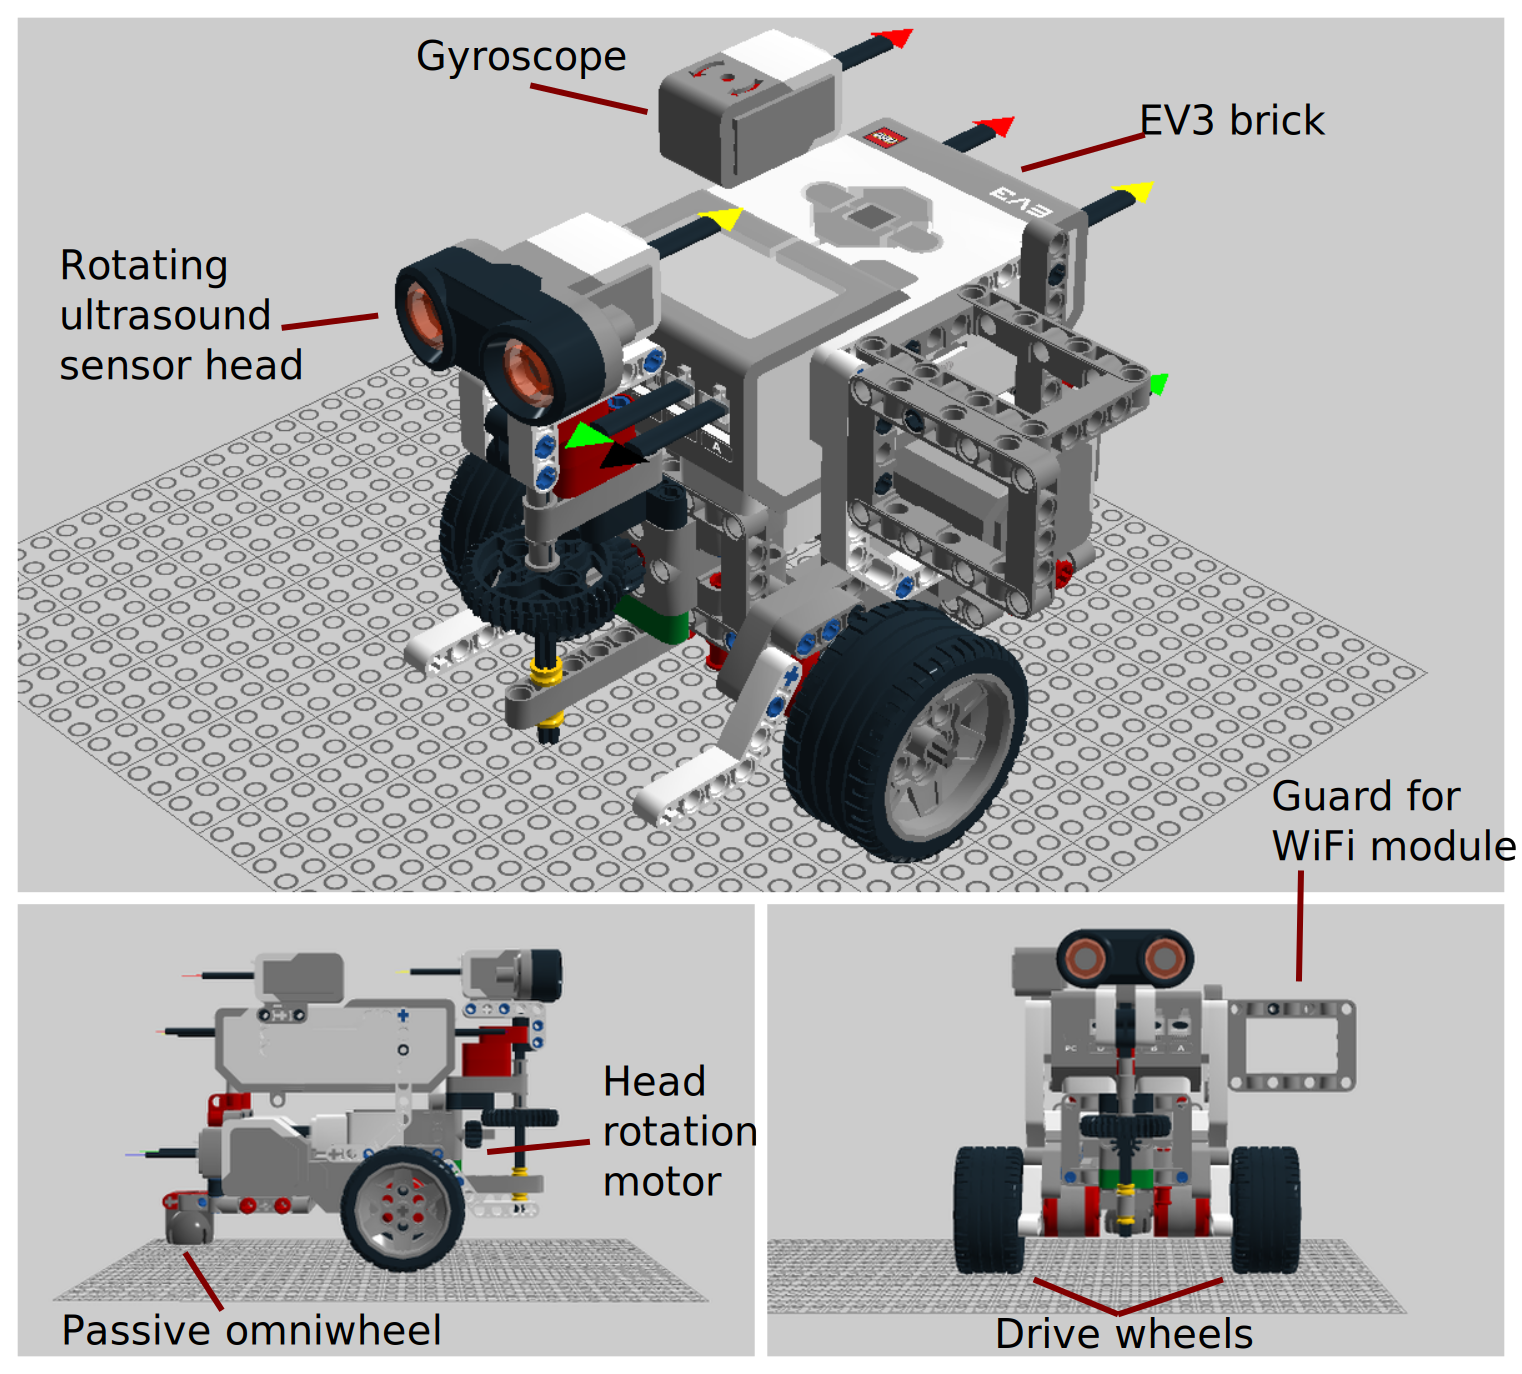
\includegraphics[width=0.9\textwidth]{fig/combined_views.pdf}
    \caption{The Lego robot used for the collaborative mapping project, rendered using the Lego Digital Designer software \cite{the_lego_group_lego_2015}.}
    \label{fig:hardware_cad}
\end{figure}

The hardware used for the mapping project is shown in Fig. \ref{fig:hardware_cad}. The design is based on plans provided by Lego for a simple two-wheeled robot, but with the addition of a rotating ultrasound sensor head, modifications to the gyroscope attachment, and a guard for the external USB WiFi module (not shown). The Lego motors for the drive wheels and the head provide absolute position encoders, and the gyroscope provides a low-drift orientation estimate. The ultrasound sensor provides an estimate of the distance from the sensor to the nearest hard surface, although its angular resolution is limited to approximately 20 degrees. 

\subsection{Software Design}

The software developed for this project can be found in three small software projects: \texttt{Ev3.jl} (low-level bindings), \texttt{Behaviors.jl} (finite-state machine behaviors), and \texttt{MappingRobots.jl} (state-estimation and point-cloud gathering). All are available on Github at \href{https://github.com/rdeits/Ev3.jl}{github.com/rdeits/Ev3.jl}, 
\href{https://github.com/rdeits/Behaviors.jl}{github.com/rdeits/Behaviors.jl}, and \href{https://github.com/rdeits/MappingRobots.jl}{github.com/rdeits/MappingRobots.jl}. 

\subsubsection{Finite-State Machine Behaviors}

The mapping robot is controlled by a set of behaviors and acts as a finite state machine. Each behavior consists of an action---a function which can be applied to the robot's motors---and a set of transitions which describe conditions for switching to another behavior. Multiple behaviors can be active simultaneously, and all active behaviors apply their individual actions to the robot's state. Only four behaviors and a start and halt state are needed to define the entire mapping task, as shown in Fig. \ref{fig:mapping_behaviors}. The general framework for defining behaviors, actions, and transitions is implemented in a standalone library, \texttt{Behaviors.jl}, created for this project. 

\begin{figure}[htbp]
    \centering
    \includegraphics[width=0.9\textwidth, clip=true, trim=1in 1in 1in 1in]{fig/behaviors.pdf}
    \caption{The behaviors used by each robot in order to explore its environment, implemented in \texttt{Behaviors.jl}. Additional timeout transitions from \texttt{Look left} and \texttt{Drive forward} to \texttt{Halt} omitted for clarity}. 
    \label{fig:mapping_behaviors}
\end{figure}

\subsubsection{Mapping}

The actual mapping code is a small set of functions built on top of the low-level bindings and the general behavior engine. At each iteration of the control loop, the code gathers data from the ultrasound and gyroscope sensors and records the absolute position of the drive and head rotation motors. That input is passed into the behavior engine, which resolves any necessary behavior transitions. The active behaviors then act on the robot's motors, causing it to drive and look in the appropriate directions to avoid obstacles and scan the environment. In addition, the change in the position of the drive wheels and the orientation of the gyroscope is used to update a dead-reckoning estimate of the robot's current position in the world. 

When the ultrasound detects a nearby object (less than 2\,m away), a single point is added to the robot's map. Over the course of exploring an environment, the robot gathers an increasingly dense pointcloud. 

\subsubsection{Parallel Collaborative Mapping}

Using Julia's built-in support for parallel computing, running multiple robots simultaneously is not much more difficult than simply running one robot. In this simple task, the robots need not share any information as they explore. Instead, each robot is initialized from a known initial position, and then it returns its entire pointcloud to the master process when its mapping behavior is complete. A collaborative mapping process, in which the robots share data to improve their maps and localization, would be a very interesting future area of work, but was beyond the scope of this project. 

Running two robots in parallel and concatenating their results is as simple as:

\begin{verbatim}
addprocs(2)
@everywhere hostnames = ["192.168.1.27", "192.168.1.25"]

maps = @sync @parallel (vcat) for i = 1:2
    robot = construct_robot(hostnames[i])
    run_mapping(robot)
end
\end{verbatim}

\section{Example Results}

\subsection{Mapping}

Using the complete Julia mapping stack, running on a host PC and communicating with the \ev{} over ZeroMQ, I was able to produce approximate maps of a set of artificial environments. The robot, built from the model shown in Fig. \ref{fig:hardware_cad} can be seen in Fig. \ref{fig:robot_in_environment}. 

\begin{figure}[htbp!]
    \centering
    \includegraphics[width=0.8\textwidth, clip=true, trim=2in 0 2in 3in]{fig/robot_in_environment.png}
    \caption{The robot exploring an environment made of cinderblocks.}
    \label{fig:robot_in_environment}
\end{figure}

Using this robot, it was possible to produce very rough maps of a simple environment constructed of cinderblocks. One such environment can be seen in Fig. \ref{fig:map_overlay}. With a second robot, it was possible to map two environments simultaneously, as seen in Fig. \ref{fig:parallel_map}. 

\begin{figure}[htbp!]
    \centering
    \begin{subfigure}[htbp]{0.45\textwidth}
        \includegraphics[width=\textwidth]{fig/N9_map_A_v1.png}
    \end{subfigure}
    \begin{subfigure}[htbp]{0.45\textwidth}
        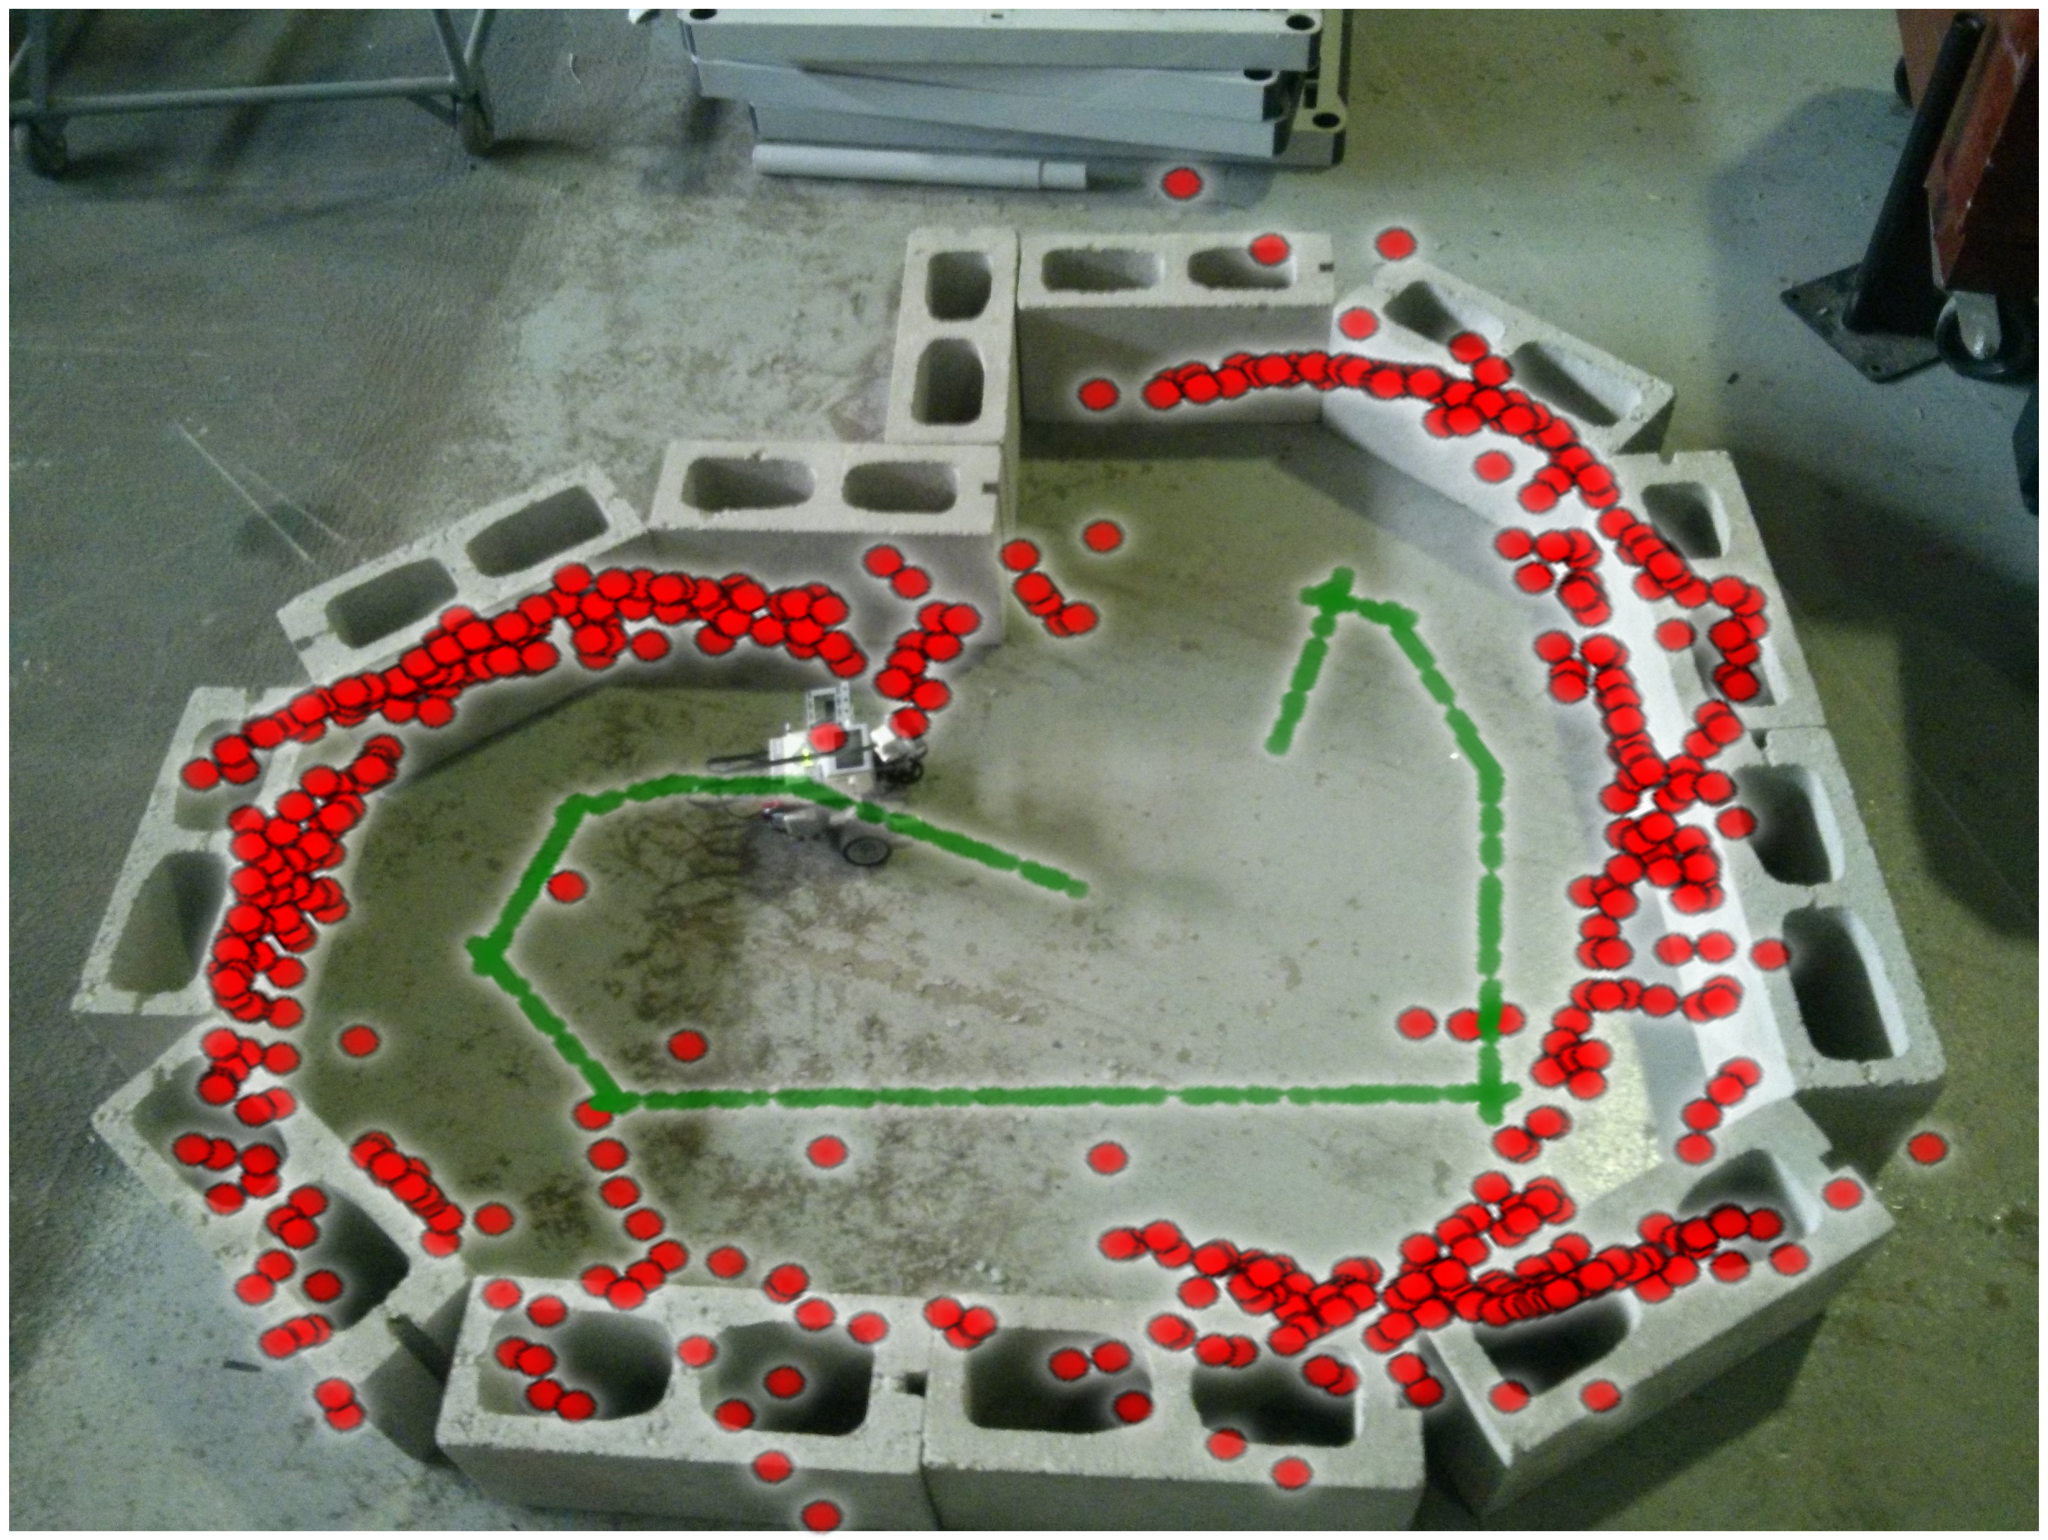
\includegraphics[width=\textwidth]{fig/map_overlay.pdf}
    \end{subfigure}
    \caption{Demonstration of the \texttt{MappingRobots.jl} package. The robot spent 120 seconds traveling around an environment made of cinderblocks. Each red point represents a single ultrasound sensor return, plotted at its x-y position in the world using the robot's estimated pose. The green path represents the robot's estimated trajectory through the world. On the right, the points have been manually overlaid (and adjusted for perspective) on top of a photo of the environment.}
    \label{fig:map_overlay}
\end{figure}

\begin{figure}[htbp!]
    \centering
    \includegraphics[width=0.8\textwidth]{fig/N9_map_A_C.png}
    \caption{Demonstration of collaborative mapping. Two robots worked simultaneously to produce the pointcloud shown here. The red points are ultrasound sensor returns, and the green paths are the robots' trajectories. The section of the left path indicated by the arrow shows a temporary loss of communication between the host PC and the \ev{} robot, during which no data about the robot's position was received.}
    \label{fig:parallel_map}
\end{figure}

\subsection{Software Performance}
\label{sec:software_performance}

The most significant problem with the mapping project is the presence of the WiFi link inside the control loop. Since the Julia mapping code is processing sensor data and producing motor commands on the host PC, it must send and receive data over WiFi at every control loop iteration. If the WiFi link is interrupted, then all control over the \ev{} robot is lost. 

In practice, running one robot at a time generally worked well, but adding a second robot resulted in frequent, temporary, losses of contact. Fortunately, the ZeroMQ layer was always able to re-establish connectivity without interrupting the task, but a total loss of motor control for several seconds is a substantial problem in a robotics application. The results of one such WiFi dropout can be seen in the very sparse data representing the left robot's estimated path in Fig. \ref{fig:parallel_map}. In order to make more complex tasks possible, it will be critical to find a way to eliminate the WiFi link from the control loop, as will be discussed in Sect. \ref{sec:future_comms}. 

\section{Future Work}

My most immediate future work will be to clean up and robustify the Julia code developed for this project so that others can use it. One important consideration is security of the Python server. As currently implemented, the server allows arbitrary files to be written and read on the \ev{} remotely by anyone on the local network. A simple way to improve this will be to restrict the server to only access the virtual files corresponding to the motors and sensors, not any other (potentially sensitive) files on the device. This will still allow any user on the user's home network to remotely control the \ev{}, but not to damage the operating system.

\subsection{Eliminating the WiFi Link}
\label{sec:future_comms}

As discussed in Sect. \ref{sec:software_performance}, the fact that every command and piece of sensor data must travel over the WiFi link is a major limitation. There are a number of possibilities that we might explore to address this. 

\subsubsection{Move Julia onto the EV3}
The most obvious way to remove the WiFi link is to remove or modify enough components of Julia to allow it to run directly on the \ev{}. With the Julia mapping code running onboard, the only communication over WiFi will be high-level, low-frequency commands, such as an instruction to start executing a mapping task. 

\subsubsection{Mount a Raspberry Pi Onboard}
If a working Julia build cannot be created for the \ev{}, there may be another way to achieve similar performance. The Raspberry Pi is a series of small, low-cost computers which run standard Linux desktop operating systems. The Raspberry Pi Zero, for example, is sold for \$5, but has 512\,MB of RAM, compared to the 64\,MB on the \ev{}, and a more modern ARMv6 architecture. There has been some success building working Julia versions for the Raspberry Pi, so it should be possible to run the mapping code on the Pi. The Pi could then be mounted directly on the robot, and could communicate with the \ev{} over USB, eliminating the unreliable WiFi link. 

\subsubsection{Replace the EV3 entirely}
Instead of adding a Raspberry Pi to the \ev{} robot, it might also be possible to replace the \ev{} brick entirely. The BrickPi is a custom device which allows Lego motors and sensors to be controlled directly by a Raspberry Pi over USB \cite{dexter_industries_brickpi_2015}. This involves some additional hardware, but might be a promising direction, since the Raspberry Pi is much more powerful than the \ev{} computer. 

\subsubsection{Robot Operating System}
Another possible direction to explore is the use of ROS, the Robot Operating System. ROS is a set of libraries for common robotics applications, including visualization, algorithms, and controls. One of the most basic elements of the ROS stack is the message-passing system, which allows different processes (potentially on different computers) to send and receive messages. It would certainly be possibly to replace the ZeroMQ layer with ROS messages over WiFi. This is unlikely to improve reliability, since the WiFi link would still be part of the control loop, but using a standardized library would make the code more likely to be compatible with other tools. There has been some very limited success getting ROS to run on the \ev{}, but as it is a very large library (hundreds of megabytes or more) and only fully supported on Ubuntu Linux, I chose not to explore it for this project. 

\section{Conclusion}

This project demonstrated a complete solution for the use of Julia to control Lego Mindstorms robots, along with an application to demonstrate Julia's excellent parallel computing facilities. While the success was limited by the intermittent communication losses over the WiFi link between the host PC and the \ev{}, it was still possible to control two robots simultaneously from the same master process. In the future, I hope to eliminate the problematic WiFi link and create more robust robotics applications. 

\bibliographystyle{IEEEtran}
\bibliography{ev3}

\end{document}